\chapter{Inżynieria danych eksperymentalnych i testowe szablony modeli}
\section{Omówienie danych eksperymentalnych}
	
	W celu zestawienia funkcjonalnego bibliotek uczenia maszynowego w języku C++ i przedstawienia przykładów konieczne było wybranie danych eksperymentalnych możliwych do wykorzystania jako porównawczy punkt odniesienia. Jako w/w dane wybrano bazę dotyczącą diagnostyki raka piersi, w której zamieszczono wyniki obrazowania określone w sposób liczbowy. Dane mają następującą strukturę:
	
	\begin{enumerate}
		\item [1)] ID - numer identyfikacyjny pacjentki;
		\item [2)] Diagnosis [\textit{Malignant - M} / \textit{Benign - B}] - charakter nowotworu, \textbf{zmienna odpowiedzi};
		\item [3)] Dane klasyfikujące:
			\begin{enumerate}
				\item [a)] \textit{Radius} - średnica guza;
				\item [b)] \textit{Texture} - tekstura guza;
				\item [c)] \textit{Perimeter} - obwód guza;
				\item [d)] \textit{Area} - pole guza;
				\item [e)] \textit{Smoothness} - gładkość, miara lokalnych różnic w promieniu guza;
				\item [f)] \textit{Compactness} - zwartość, wykorzystywana do oceny stadium guza;
				\item [g)] \textit{Concavity} - stopień wklęsłości miejsc guza;
				\item [h)] \textit{Concave points} - punkty wklęsłości guza;
				\item [i)] \textit{Symmetry} - symetria guza, pomagająca w ocenie charakteru przyrostu guza.
				\item [j)] \textit{Fractal dimention (,,coastline approximation'' - 1)} - wymiar fraktalny pozwalający na ilościowy opis złożoności komórek nerwowych, umożliwiający stwierdzenie nowotworzenia się zbioru komórek.
			\end{enumerate}
	\end{enumerate}
	
	Dla każdej ze zmiennych odpowiedzi została zebrana średnia wartość, odcyhelenie standardowe oraz średnia trzech największych pomiarów, gdzie każdy zestaw ustawiony jest sekwencyjnie (np. kolumna 3 - średni promień, kolumna 12 - odchylenie standardowe promienia, kolumna 22 - średnia trzech największych pomiarów promienia). Każda ze zmiennych ma charakter ciągły.
	
\section{Charakterystyka i przetwarzenie danych}

	W celu przeprowadzenia procesu uczenia maszynowego, jednym z najistotniejszych kroków jakie należy podjąć jest wstępne zaznajomienie się z zestawem danych i jego analiza pod kątem rozkładu poszczególnych zmiennych oraz prawdopodobieństw. W tym celu wykorzystane zostało oprogramowanie JMP. 

	\subsection{Analiza rozkładu danych}
	
	\begin{figure}[!ht]
		\centering
		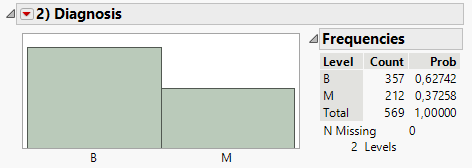
\includegraphics[width=0.8\linewidth]{Rysunki/Rozdzial2/diagnosis_distribution}
		\caption{Histogram rozkładu zmiennej odpowiedzi}
		\label{fig:diagnosisdistribution}
	\end{figure}
	
	\begin{figure}[!ht]
		\centering
		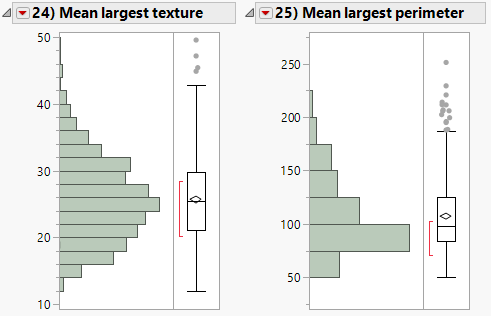
\includegraphics[width=0.7\linewidth]{Rysunki/Rozdzial2/variable_distribution}
		\caption{Przykłady histogramów zmiennych decyzyjnych}
		\label{fig:variabledistribution}
	\end{figure}
	
	
	Proces analizy rozkładu rozpoczęty został od przyjrzenia się zmiennej odpowiedzi (\textit{Diagnosis}). Rysunek 3.1 przedstawia uzyskany histogram, wraz z tabelą określającą ilość obserwacji danej klasy i współczynnik prawdopodobieństwa przynależności odpowiedzi do danej klasy. Zauważyć można, że dla użytego zestawu danych ilość zarejestrowano 357 obserwacji łagodnego raka piersi, a jego prawdopodobieństwo przynależności do klasy \textit{Benign} wynosi $\approx$ 62,7\%, natomiast do klasy \textit{Malignant} przynależało 212 obserwacji z prawodpodobieństwem $\approx$ 37,3\%.
		
	Podczas analizy histogramów zmiennych decyzyjnych, stwierdzono że znaczna ilość ma charakter prawostronnie skośny oraz występują dla nich obserwacje odstające, o czym informuje znajdujący się po prawej stronie histogramu wykres okienkowy (ang. \textit{box graph}), co przedstawiono na rysunku 3.2. Wyjątkiem okazała się zmienna \textit{Mean Largest Concave Points}), która mimo lekkiej skośności, okazała się nie posiadać obserwacji odstających. Na podstawie tych informacji stwierdzono, że aby przygotować dane w odpowiedni sposób do procesu uczenia należy przeprowadzić ich czyszczenie oraz normalizację.
	
	\subsection{Czyszczenie danych}
	
	Na pełny zestaw danych składa się 569 obserwacji. Podczas wstępnej analizy nie stwierdzono istnienia brakujących wartości, w związku z czym głównym problemem okazały się obserwacje odstające. Do usunięcia obserwacji odstających wykorzystano wykresy okienkowe, gdzie oś Y reprezentowała zmienną odpowiedzi, natomiast oś X czyszczoną zmienną decyzyjną. Pozwoliło to na zachowanie relatywnego stosunku poszczególnych klas (co okazało się niemożliwe przy pierwszej próbie usunięcia wprost obserwacji odstających bez uwzględnienia poszczególych klas, skutkując w prawie całkowitym wyeliminowaniu klasy \textit{Malignant}). Przykładowy wykres został przedstawiony na rysunku 3.3.
	
	\begin{figure}[!ht]
		\centering
		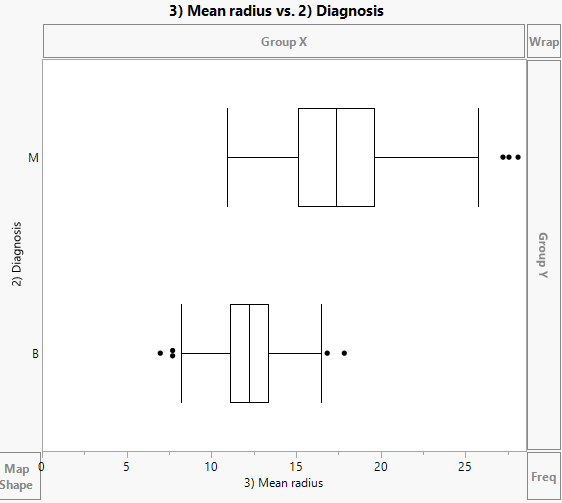
\includegraphics[width=0.7\linewidth]{Rysunki/Rozdzial2/box_graph}
		\caption{Przykład analizy obserwacji odstających dla poszczególnych klas zmiennej odpowiedzi}
		\label{fig:boxgraph}
	\end{figure}

	\newpage
	

\section{Szablony docelowych modeli dla zadanych danych eksperymentalnych}

Ze względu na dychotomiczny charakter zmiennej odpowiedzi, wybrany został przedstawiony poniżej zestaw metod dla których wykonano i przedstawiono testy praktyczne. Szablony struktury rozwiązań, takie jak np. wybór zmiennych uczestniczących w procesie uczenia, lub struktura sieci neuronowej zostały ustalone w sposób empiryczny z wykorzystaniem programu do uczenia maszynowego JMP. 

\subsection{Regresja logistyczna}

\subsection{Głęboka sieć neuronowa}

\subsection{Maszyna wektorów nośnych}